\documentclass[tikz]{standalone}

\begin{document}
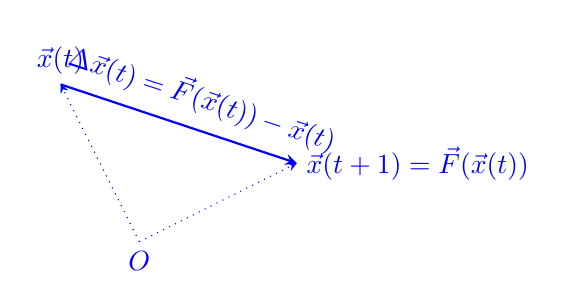
\begin{tikzpicture}
  \draw[->,>=stealth,blue,dotted] (0,0)--(-1,2) node[above]{\(\vec{x}(t)\)};		
  \draw[->,>=stealth,blue,dotted] (0,0)--(2,1) node[right]{\(\vec{x}(t+1)=\vec{F}(\vec{x}(t))\)};
  \draw[->,>=stealth,blue,thick] (-1,2)--(2,1);
  \node[above,rotate=-18,blue] at (0.7,1.5) {\(\Delta\vec{x}(t)=\vec{F}(\vec{x}(t)) - \vec{x}(t)\)};
  \node[below,blue] at (0,0) {\(O\)};
\end{tikzpicture}
\end{document}
